\section{The Analysis of Security and Privacy}
\label{sec:analysis}
In this section, we presents the analysis that UPPRESSO achieves the required properties of security and privacy.


\subsection{Security}
UPPRESSO satisfies the four security requirements of identity tokens in SSO services,
     as listed in Section \ref{subsec:basicrequirements}.

%while the detailed process of proof is provided in the Appendix.
% ����汾���Ȳ��ܸ�¼��

\vspace{1mm}
\noindent\textbf{RP Designation.}
An identity token binding $PID_U$ and $PID_{RP}$,
    designates the target RP, and only the target RP.
An honest RP calculates $PID_{RP}$ by itself with the trapdoor $t$ sent from the user,
    and checks $PID_{RP}$ in the $PID_{RP}$-registration result and the identity token.
So the target RP will accept this token.

Meanwhile,
        the honest IdP guarantees that, within its validity period, the $PID_{RP}$ will be registered only once.
% $PID_{RP}$ will be bound in some identity token.
An honest RP is ready to accept an identity token binding $PID_{RP}$, only after it receives the signed $PID_{RP}$-registration result.
Because both $PID_{RP}$ and $H(t)$ in the registration result are checked by the RP and then the registration result $[PID_{RP}, H(t), Validity]_{SK}$ is acceptable to only one honest RP,
            the identity token designates only one RP.

\vspace{1mm}
\noindent\textbf{User Identification.}
An honest RP always derives an identical permanent account from different identity tokens binding $PID_U$ and $PID_{RP}$.
That is,
    in the user's any $i$-th and $i'$-th ($i \neq i'$) login instances to the RP,
 $\mathcal{F}_{Acct}(PID_{U}^i, PID_{RP}^i) = \mathcal{F}_{Acct}(PID_{U}^{i'}, PID_{RP}^{i'}) = [ID_U]ID_{RP}$.

In the calculation of $Acct = [t^{-1}]PID_U = [t^{-1}][u]PID_{RP}$,
$t$ and $PID_{RP}$ have been checked by the honest RP in the $PID_{RP}$-registration result,
    and $PID_U$ is calculated by the honest IdP based on (\emph{a}) the authenticated user, i.e., $ID_U = u$,
            and (\emph{b}) the registered $PID_{RP}$.
Thus, the calculated account is always exactly the authenticated user's account at the RP (i.e., $[ID_U]ID_{RP}$).
For example,
    two malicious users, whose identities are $ID_U = u$ and $ID_{U'} = u'$,
    could attempt to login to $RP_j$ and $RP_{j'}$, respectively.
If the generated $t$ and $t'$ happen to satisfy that $PID_{RP} = [t]ID_{RP_j} = [tr]G = [t'r']G = [t']ID_{RP_{j'}}$,
    these collusive users could arbitrarily choose to register either $[PID_{RP}, PEnpt_U, H(t)]$ or $[PID_{RP}, PEnpt_{U'}, H(t')]$ at the IdP,
        to receive an identity token binding either $PID_U = [u]PID_{RP}$ or $PID_{U'} = [u']PID_{RP}$
         (and also $PID_{RP}$).\footnote{Such a token designates either $RP_j$ or $RP_{j'}$,
    but only one honest RP because there is only one acceptable $PID_{RP}$-registration result which is signed by the IdP.
    So RP designation is not violated in this case.}
However,
    when such a token is signed for $RP_j$, the calculated $Acct$ is $[ur]G$ or $[u'r't't^{-1}]G = [u'r]G$;
    when it is signed for $RP_{j'}$, $[urtt'^{-1}]G = [ur']G$ or $[u'r']G$ is calculated.
That is,
        even in this collusive case,
    the calculated account is still the authenticated user's account at the RP,
    and it does not result in any attack.


%An adversary might try allure a user to login under the adversary's account,
%    by injecting his identity token into the user's communications with an honest RP.
%Such identity injection attacks are impossible in UPPRESSO as follows.
%If the negotiation of $PID_{RP}$ is not finished yet,
%    the RP will reject the malicious token.
%Even when $PID_{RP}$ has been negotiated,
%    it is kept unknown to the adversary because the communications between two scripts are controlled by a browser
%     and the communications between the browser and the IdP (or the RP) are protected by TLS.
%Thus, an adversary cannot obtain $PID_{RP}$ dynamically negotiated between an honest RP and the user,
%     so it cannot construct an identity token acceptable to the RP.
%

\vspace{1mm}
\noindent\textbf{Confidentiality.}
There is no event leaking the identity tokens to any malicious entity other than the authenticated user and the designated RP.
First of all, the communications among the IdP, RPs and users,
    are protected by HTTPS,
    and the \verb+postMessage+ HTML5 API ensures the dedicated channels between two scripts within the browser,
    so that adversaries cannot eavesdrop the identity tokens.
Meanwhile, the honest IdP sends the identity token only to the authenticated user,
    and this user forwards it to the RP through $Enpt_{RP}$.
The binding of $Enpt_{RP}$ and $ID_{RP}$ is ensured by the signed RP certificate,
so only the designated target RP receives this identity token.
%The detailed process of proof is shown in Appendix.

\vspace{1mm}
\noindent\textbf{Integrity.}
The identity token binds $ID_U$ and $ID_{RP}$
    implicitly, and any breaking will result in some failed check or verification in the login flow.
The integrity is ensured by the IdP's signatures:
 (\emph{a}) the identity token binding $PID_U$ and $PID_{RP}$, is signed by the IdP,
  and (\emph{b}) the relationship between $PID_{RP}$ and $t$ (or collision-free $H(t)$) is also bound
    in the $PID_{RP}$-registration result.
Thus,
    $ID_U$ and $ID_{RP}$ are actually bound by the IdP's signatures,
        due to the one-to-one mapping between (\emph{a}) the pair of $ID_U$ and $ID_{RP}$ and (\emph{b}) the triad of $PID_U$, $PID_{RP}$, and $t$.

%The detailed process of proof is shown in Appendix.

%The detailed process of proof is shown in Appendix.

\vspace{1mm}
We also formally analyze the security properties of UPPRESSO,
     based on an Dolev-Yao style model of the web infrastructure \cite{SPRESSO},
 which has been used in the formal analysis of SSO protocols such as OAuth 2.0 \cite{FettKS16} and OIDC \cite{FettKS17}.
The Dolev-Yao style model abstracts the entities in a web system,
    such as browsers and web servers,
    as {\em atomic processes}, which communicate with each other through {\em events}.
It also defines {\em script processes} to formulate client-side scripts, i.e.,  JavaScript code,
 so a web system consists of a set of atomic and script processes.

The UPPRESSO system contains an IdP process,
    a finite set of web servers for honest RPs, a finite set of honest browsers, and a finite set of attacker processes.
Here, we consider all RP processes and browser processes are honest,
 while model an RP or a browser controlled by an adversary as atomic attacker processes.
It also contains {\sf script\_rp}, {\sf script\_idp} and {\sf script\_attacker},
    where {\sf script\_rp} and {\sf script\_idp} are honest scripts downloaded from an RP process and the IdP process, respectively,
         and {\sf script\_attacker} denotes a script downloaded by an attacker process that exists in all browser processes.

After formulating UPPRESSO by the Dolev-Yao style model,
    we trace the identity token,
        starting when it is generated and ending when consumed,
 to ensure that an identity token is not leaked or tampered with.
We locate the generation of an identity token in UPPRESSO, and trace back to the places
    where $PID_U$, $PID_{RP}$ and other values enclosed in this token are generated and transmitted,
     to ensure that no adversary is able to retrieve or manipulate them.
The tracing of identity tokens also confirm no adversary retrieves the token.

Finally,
    we formally prove that,
\emph{user identification}, \emph{RP designation}, \emph{confidentiality}, and \emph{integrity} are fulfilled in UPPRESSO.
The details on the Dolev-Yao web model and the security proofs of UPPRESSO are in the appendix.





\subsection{Privacy}
We show that UPPRESSO effectively prevents the attacks of IdP-based login tracing and RP-based identity linkage.

\vspace{1mm}
\noindent\textbf{IdP-based Login Tracing.}
The information accessible to the IdP and derived from the RP's identity,
    is only $PID_{RP}$, where $PID_{RP} = [t]ID_{RP}$ is calculated by the user.
Because  (\emph{a}) $t$ is a number randomly chosen from $(1,n)$ by the user and kept secret to the IdP
 and (\emph{b}) $ID_{RP} = [r]G$ and $G$ is the base point (or generator) of $\mathbb{E}$,
 the IdP has to view $PID_{RP}$ as randomly and independently chosen from $\mathbb{E}$,
    and cannot distinguish $[t]ID_{RP_j} = [tr]G$ from $[t']ID_{RP_{j'}} = [t'r']G$.
So, the IdP cannot derive the RP's identity or link any pair of $PID_{RP}^i$ and $PID_{RP}^{i'}$,
    and then the IdP-based identity linkage is impossible.

\vspace{1mm}
\noindent\textbf{RP-based Identity Linkage.}
We prove that UPPRESSO prevents the RP-based identity linkage,
 based on the elliptic curve decision Diffie-Hellman (ECDDH) assumption \cite{GoldwasserK16}.
%We briefly introduce the ECDDH assumption.

Let $\mathbb{E}$ be an elliptic curve over a finite field $\mathbb{F}_q$,
    and $P$ be a point on $\mathbb{E}$ of order $n$.
For any probabilistic polynomial time (PPT) algorithm $\mathcal{D}$,
 $([x]P$, $[y]P$, $[xy]P)$ and $([x]P$, $[y]P$, $[z]P)$
are computationally indistinguishable,
 where $x$, $y$ and $z$ are integer numbers randomly and independently chosen from $(1,n)$.
Let  $Pr\{\}$ denote the probability and
 we define
\begin{align*}
Pr_1 = & Pr\{\mathcal{D}(P, [x]P, [y]P, [xy]P)=1\} \\
Pr_2 = & Pr\{\mathcal{D}(P, [x]P, [y]P, [z]P)=1\} \\
\epsilon(k) = & Pr_1 - Pr_2
\end{align*}
Then, $\epsilon(k)$ becomes negligible with the security parameter $k$.

%Let $q$ be a large prime and $\mathbb{G}$ denotes a cyclic group of order $n$ of an elliptic curve $E(\mathbb{F}_q)$.
%Assume that $n$ is also a large prime. Let $P$ be a generator point of $\mathbb{G}$.

%where $q$ and $n$ are large primitive number, and $P$ is the point of $\mathbb{G}$.
%For any probabilistic polynomial time (PPT) algorithm $D$, the distributions, \{$P$, $aP$, $bP$, $abP$\}$_{a,b \in \mathbb{Z}_n}$ and \{$P$, $aP$, $bP$, $cP$\}$_{a,b,c \in \mathbb{Z}_n}$, are computationally indistinguishable. There is a negligible $\sigma(k)$, where $k$ is the security parameter.

In the login flow,
    an RP holds $ID_{RP}$ and $Acct$, receives $t$, calculates $PID_{RP}$,
    and verifies two signed messages (i.e., $PID_{RP}$ and $H(t)$ in the $PID_{RP}$-registration result,
            and $PID_{RP}$ and $PID_U$ in the identity token).
After filtering out the redundant information (i.e., $PID_{RP}= [t]{ID_{RP}}$ and $Acct = [t^{-1}]PID_{U}$),
    the RP actually receives only $(ID_{RP}, t, PID_U)$ in each SSO login instance, where $PID_U = [ID_U][t]{ID_{RP}}$.

% ���̫���ˣ�����Ҫͼ
%\begin{figure*}
%  \centering
%  \includegraphics[width=0.82\linewidth]{fig/game1.pdf}
%  \caption{The Game.}
%  \label{fig:game}
%\end{figure*}


In the RP-based identity linkage,
    two RPs bring two triads received in SSO login instances, $(ID_{RP_j}$, $t_j$, $[ID_U][t_j]{ID_{RP_j}})$ and
    $(ID_{RP_{j'}}$, $t_{j'}$, $[ID_{U'}] [t_{j'}] {ID_{RP_{j'}}})$.
We describe the attack as the following game $\mathcal{G}$ between an adversary and a challenger:
    the adversary receives $(ID_{RP_j}$, $t_j$, $[ID_U][t_j]{ID_{RP_j}}, ID_{RP_{j'}}$, $t_{j'}$, $[ID_{U'}] [t_{j'}] {ID_{RP_{j'}}})$ from the challenger,
     and outputs the result $s$.
The result is 1, when the adversary guesses that $ID_U = ID_{U'}$;
     otherwise, the adversary thinks they are different users (i.e., $ID_U \neq ID_{U'}$) and $s=0$.
%The game is shown as Figure \ref{fig:game}.

We define $Pr_c$ as the probability that
    the adversary outputs $s=1$ when $ID_U = ID_{U'}$ (i.e., a \emph{correct} identity linkage),
    and $Pr_{\bar{c}}$ as the probability that $s=1$ but $ID_U \neq ID_{U'}$ (i.e., an \emph{incorrect} result).
The successful RP-based identity linkage means
    the adversary has non-negligible advantages in $\mathcal{G}$.

\begin{figure}[tb]
  \centering
  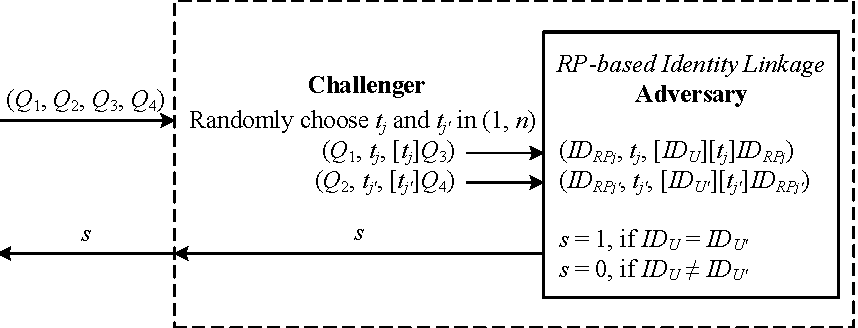
\includegraphics[width=0.95\linewidth]{fig/dalgorithm.pdf}
  \caption{The algorithm based on the RP-based identity linkage, to solve the ECDDH problem.}
  \label{fig:dalgorithm}
\end{figure}

We design a PPT algorithm $\mathcal{D}^*$ based on $\mathcal{G}$, shown in Figure \ref{fig:dalgorithm}.
The input of $\mathcal{D}^*$ is in the form of $(Q_1, Q_2, Q_3, Q_4)$, and each $Q_i$ is a point on $\mathbb{E}$.
On receiving the input,
 the challenger of $\mathcal{G}$ randomly chooses $t_j$ and $t_{j'}$ in $(1,n)$,
   % and sets $ID_{RP_j}=Q_1$, $ID_{RP_{j'}}=Q_2$, $PID_{U,j}=[t_j]Q_3$, and $PID_{U',j'}= [t_{j'}] Q_4$.
    and sends $(Q_1, t_j, [t_j]Q_3, Q_2, t_{j'}, [t_{j'}] Q_4)$ to the adversary.
Finally,
    it directly outputs $s$ from the adversary in $\mathcal{G}$ as the result of $\mathcal{D}^*$.

Let ($P$, $[x]P$, $[y]P$, $[xy]P$) and  ($P$, $[x]P$, $[y]P$, $[z]P$) be two inputs of $\mathcal{D}^*$.
Thus, we obtain
\begin{equation}\label{eq:game-succed}
\begin{split}
&Pr\{\mathcal{D}^*(P,[x]P,[y]P,[xy]P)=1\}\\
=&Pr\{\mathcal{G}(P, t_j, [t_j][y]P, [x]P, t_{j'},[t_{j'}][xy]P)=1\}\\
=&Pr\{\mathcal{G}(P, t_j, [y][t_j]P, [x]P, t_{j'},[y][t_{j'}][x]P)=1\}=Pr_c
\end{split}
\end{equation}
\begin{equation}\label{eq:game-fail}
\begin{split}
&Pr\{\mathcal{D}^*(P,[x]P,[y]P,[z]P)=1\} \\
=&Pr\{\mathcal{G}(P, t_j, [t_j][y]P, [x]P, t_{j'},[t_{j'}][z/x] [x]P)=1\}\\
=&Pr\{\mathcal{G}(P, t_j, [y][t_j]P, [x]P, t_{j'},[z/x][t_{j'}][x]P)=1\}=Pr_{\bar{c}}
\end{split}
\end{equation}
Equation \ref{eq:game-succed} is equal to $Pr_c$
        because it represents the correct case of $ID_{U} = ID_{U'} = y$,
 while Equation \ref{eq:game-fail} is $Pr_{\bar{c}}$ for it represents the incorrect case of $ID_{U} =y$ but $ID_{U'} = z/x \bmod n$.


The adversary has non-negligible advantages in $\mathcal{G}$ means
    $Pr_c - Pr_{\bar{c}}>\sigma(k)$,
    and then $\mathcal{D}^*$ significantly distinguishes ($P$, $[x]P$, $[y]P$, $[xy]P$) from  ($P$, $[x]P$, $[y]P$, $[z]P$),
    which violates the ECDDH assumption.
So the adversary has no advantages in the game,
    and the RP-based identity linkage is computationally impossible in UPPRESSO.
